\chapter{System Design and Implementation}
\label{ch:system_design_implementation}

This chapter presents the core architecture of SENTINEL. The two-tier design decisively resolves the performance bottlenecks associated with Generative AI in cybersecurity.

\section{Two-Tier Architecture Overview}
SENTINEL segregates the processing pipeline into two specialized tiers (Figure~\ref{fig:soc_ai_concept}).
\textbf{Tier-1:} Operates at high-speed network edges, utilizing Regex rules and the Welford algorithm for anomaly detection. A Machine Learning Gateway (LightGBM) classifies and resolves the majority of alerts, escalating only complex, ambiguous cases to Tier-2.
\textbf{Tier-2:} A locally hosted Agentic AI (Gemma-9B) references a knowledge base (RAG) and Threat Memory to make structured mitigation decisions (Block, Alert, Drop, HITL).

\begin{figure}[!htbp]
    \centering
    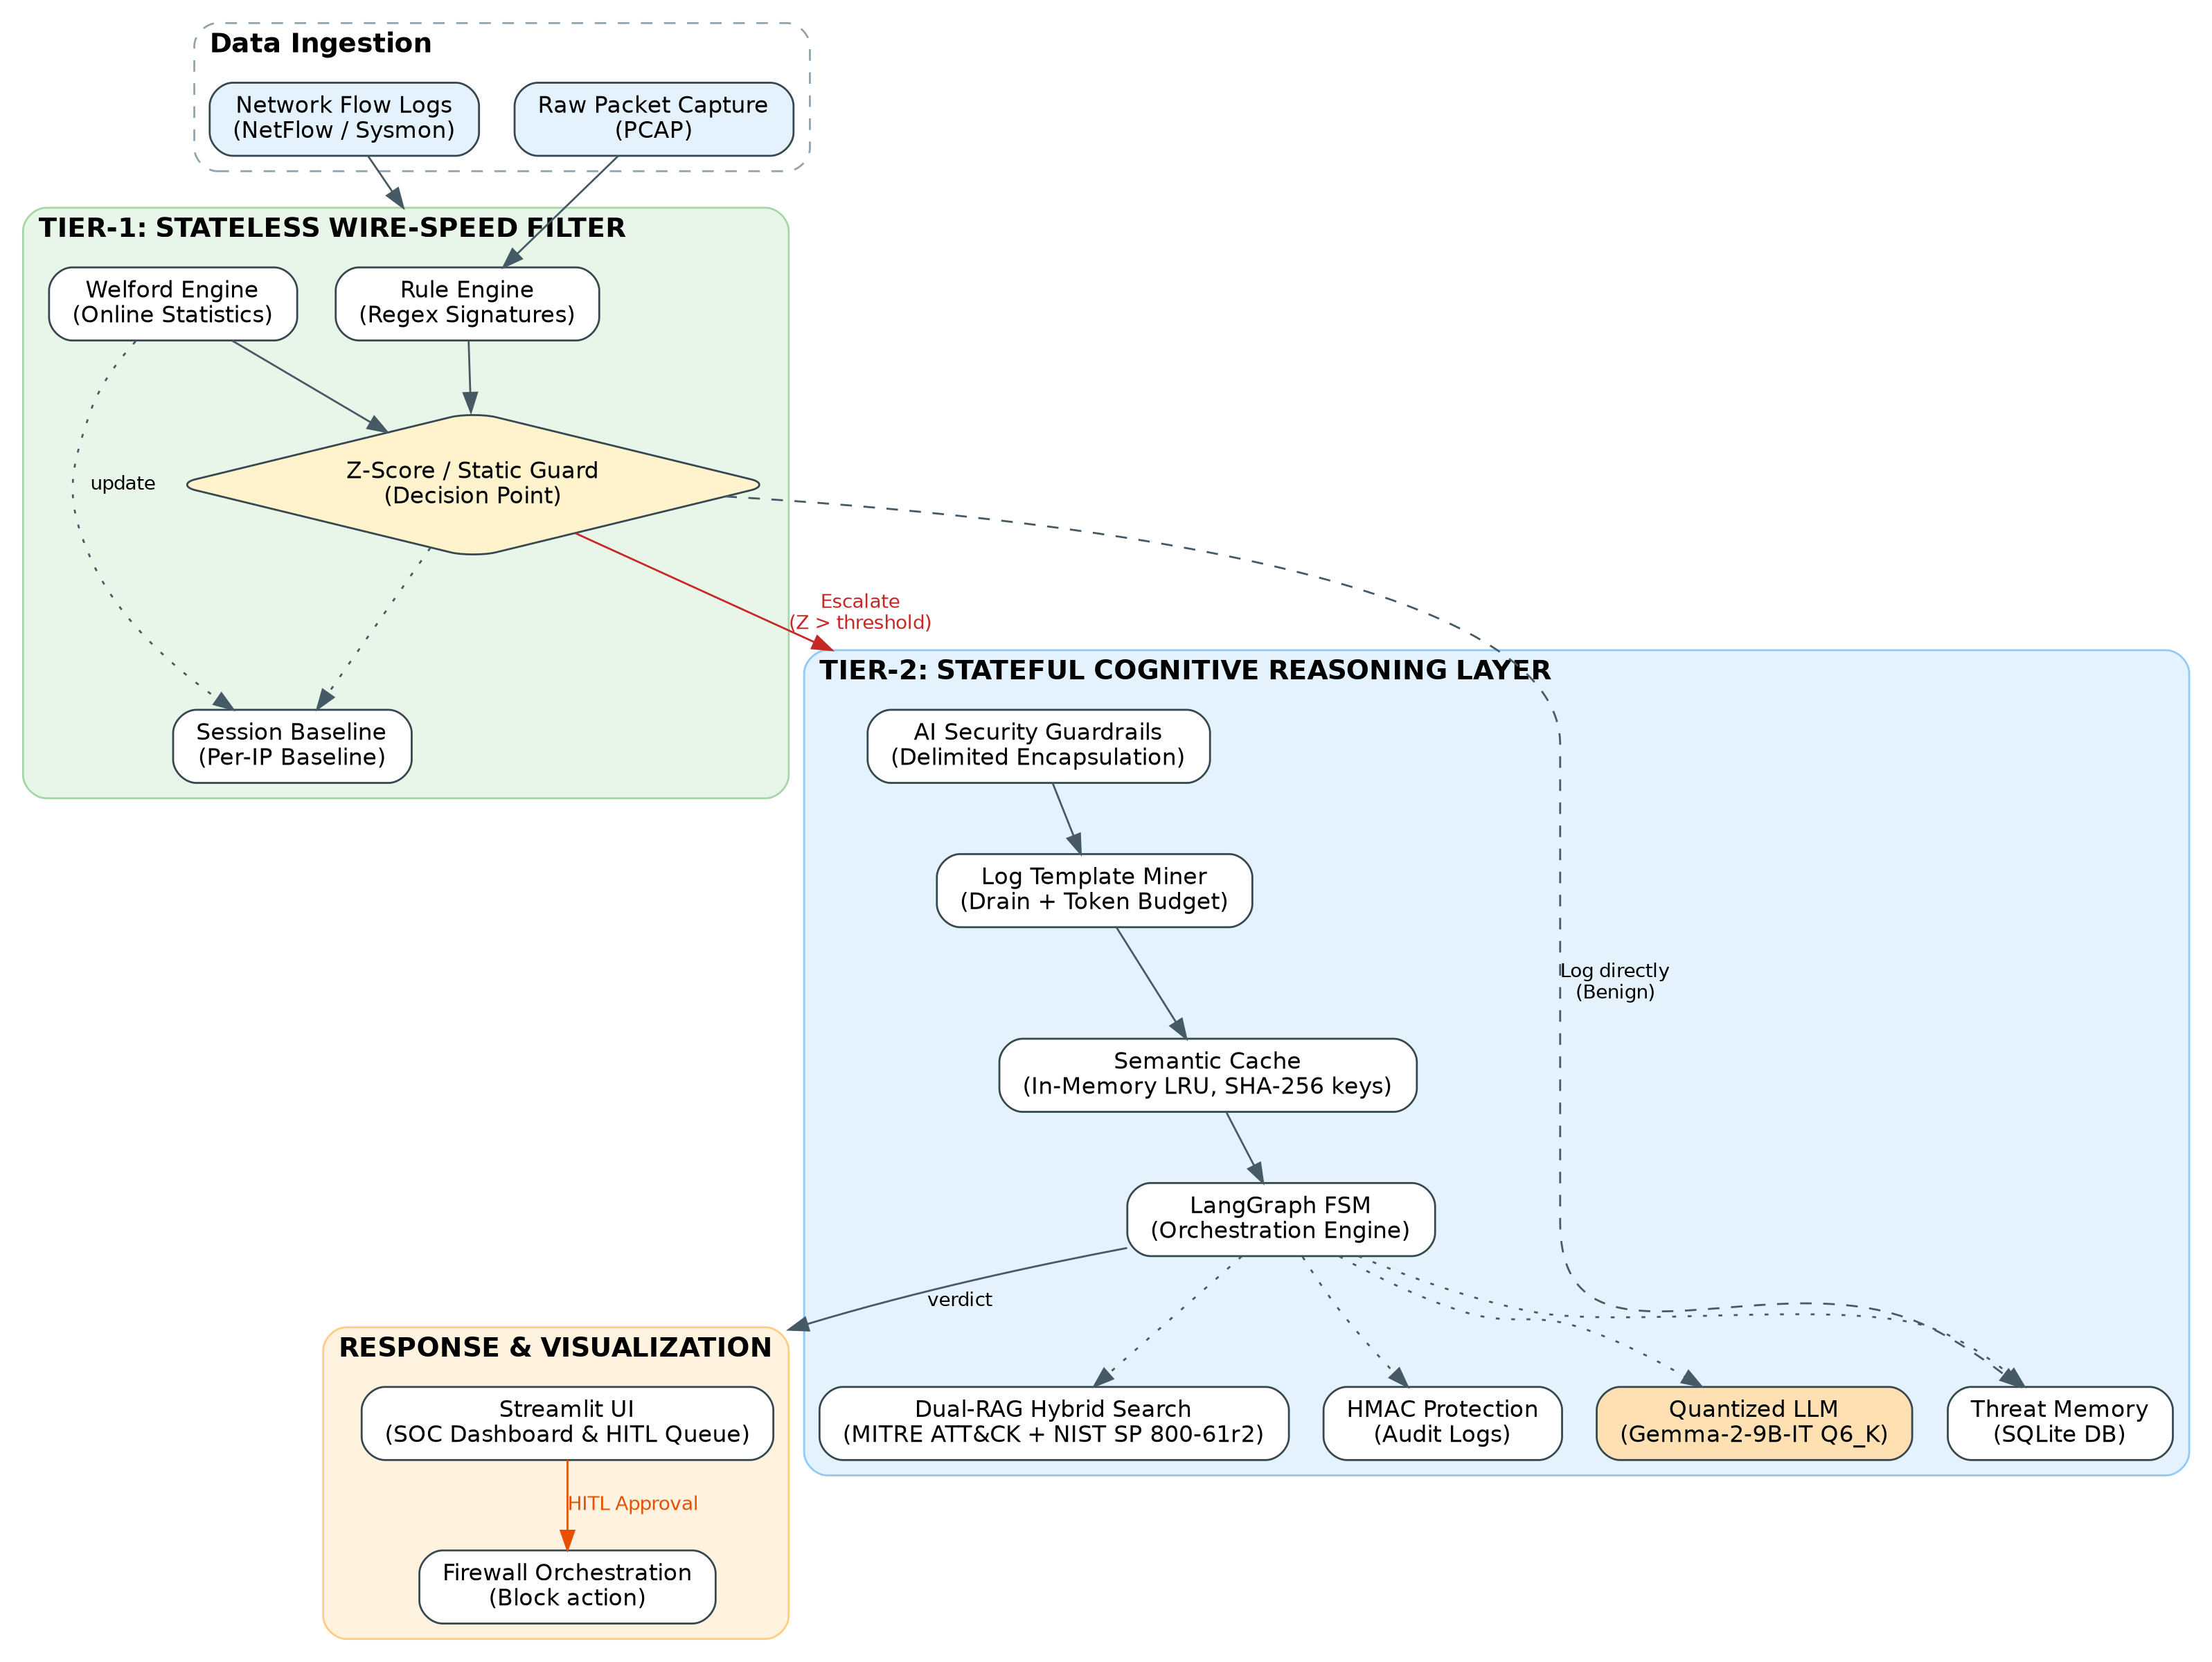
\includegraphics[width=0.95\textwidth,height=0.66\textheight,keepaspectratio]{images/soc_ai_concept.png}
    \caption{SENTINEL Overall Architecture: two-tier data flow and components. (Source: Author)}
    \label{fig:soc_ai_concept}
\end{figure}

The operational flow (Figure~\ref{fig:sentinel_flow}) ensures transparency. Logs bypassing the Tier-1 filter are scored by the ML Gateway. Uncertain cases are securely enclosed within "Guardrails", enriched via RAG, and passed to the LLM for final adjudication.

\begin{figure}[!htbp]
    \centering
    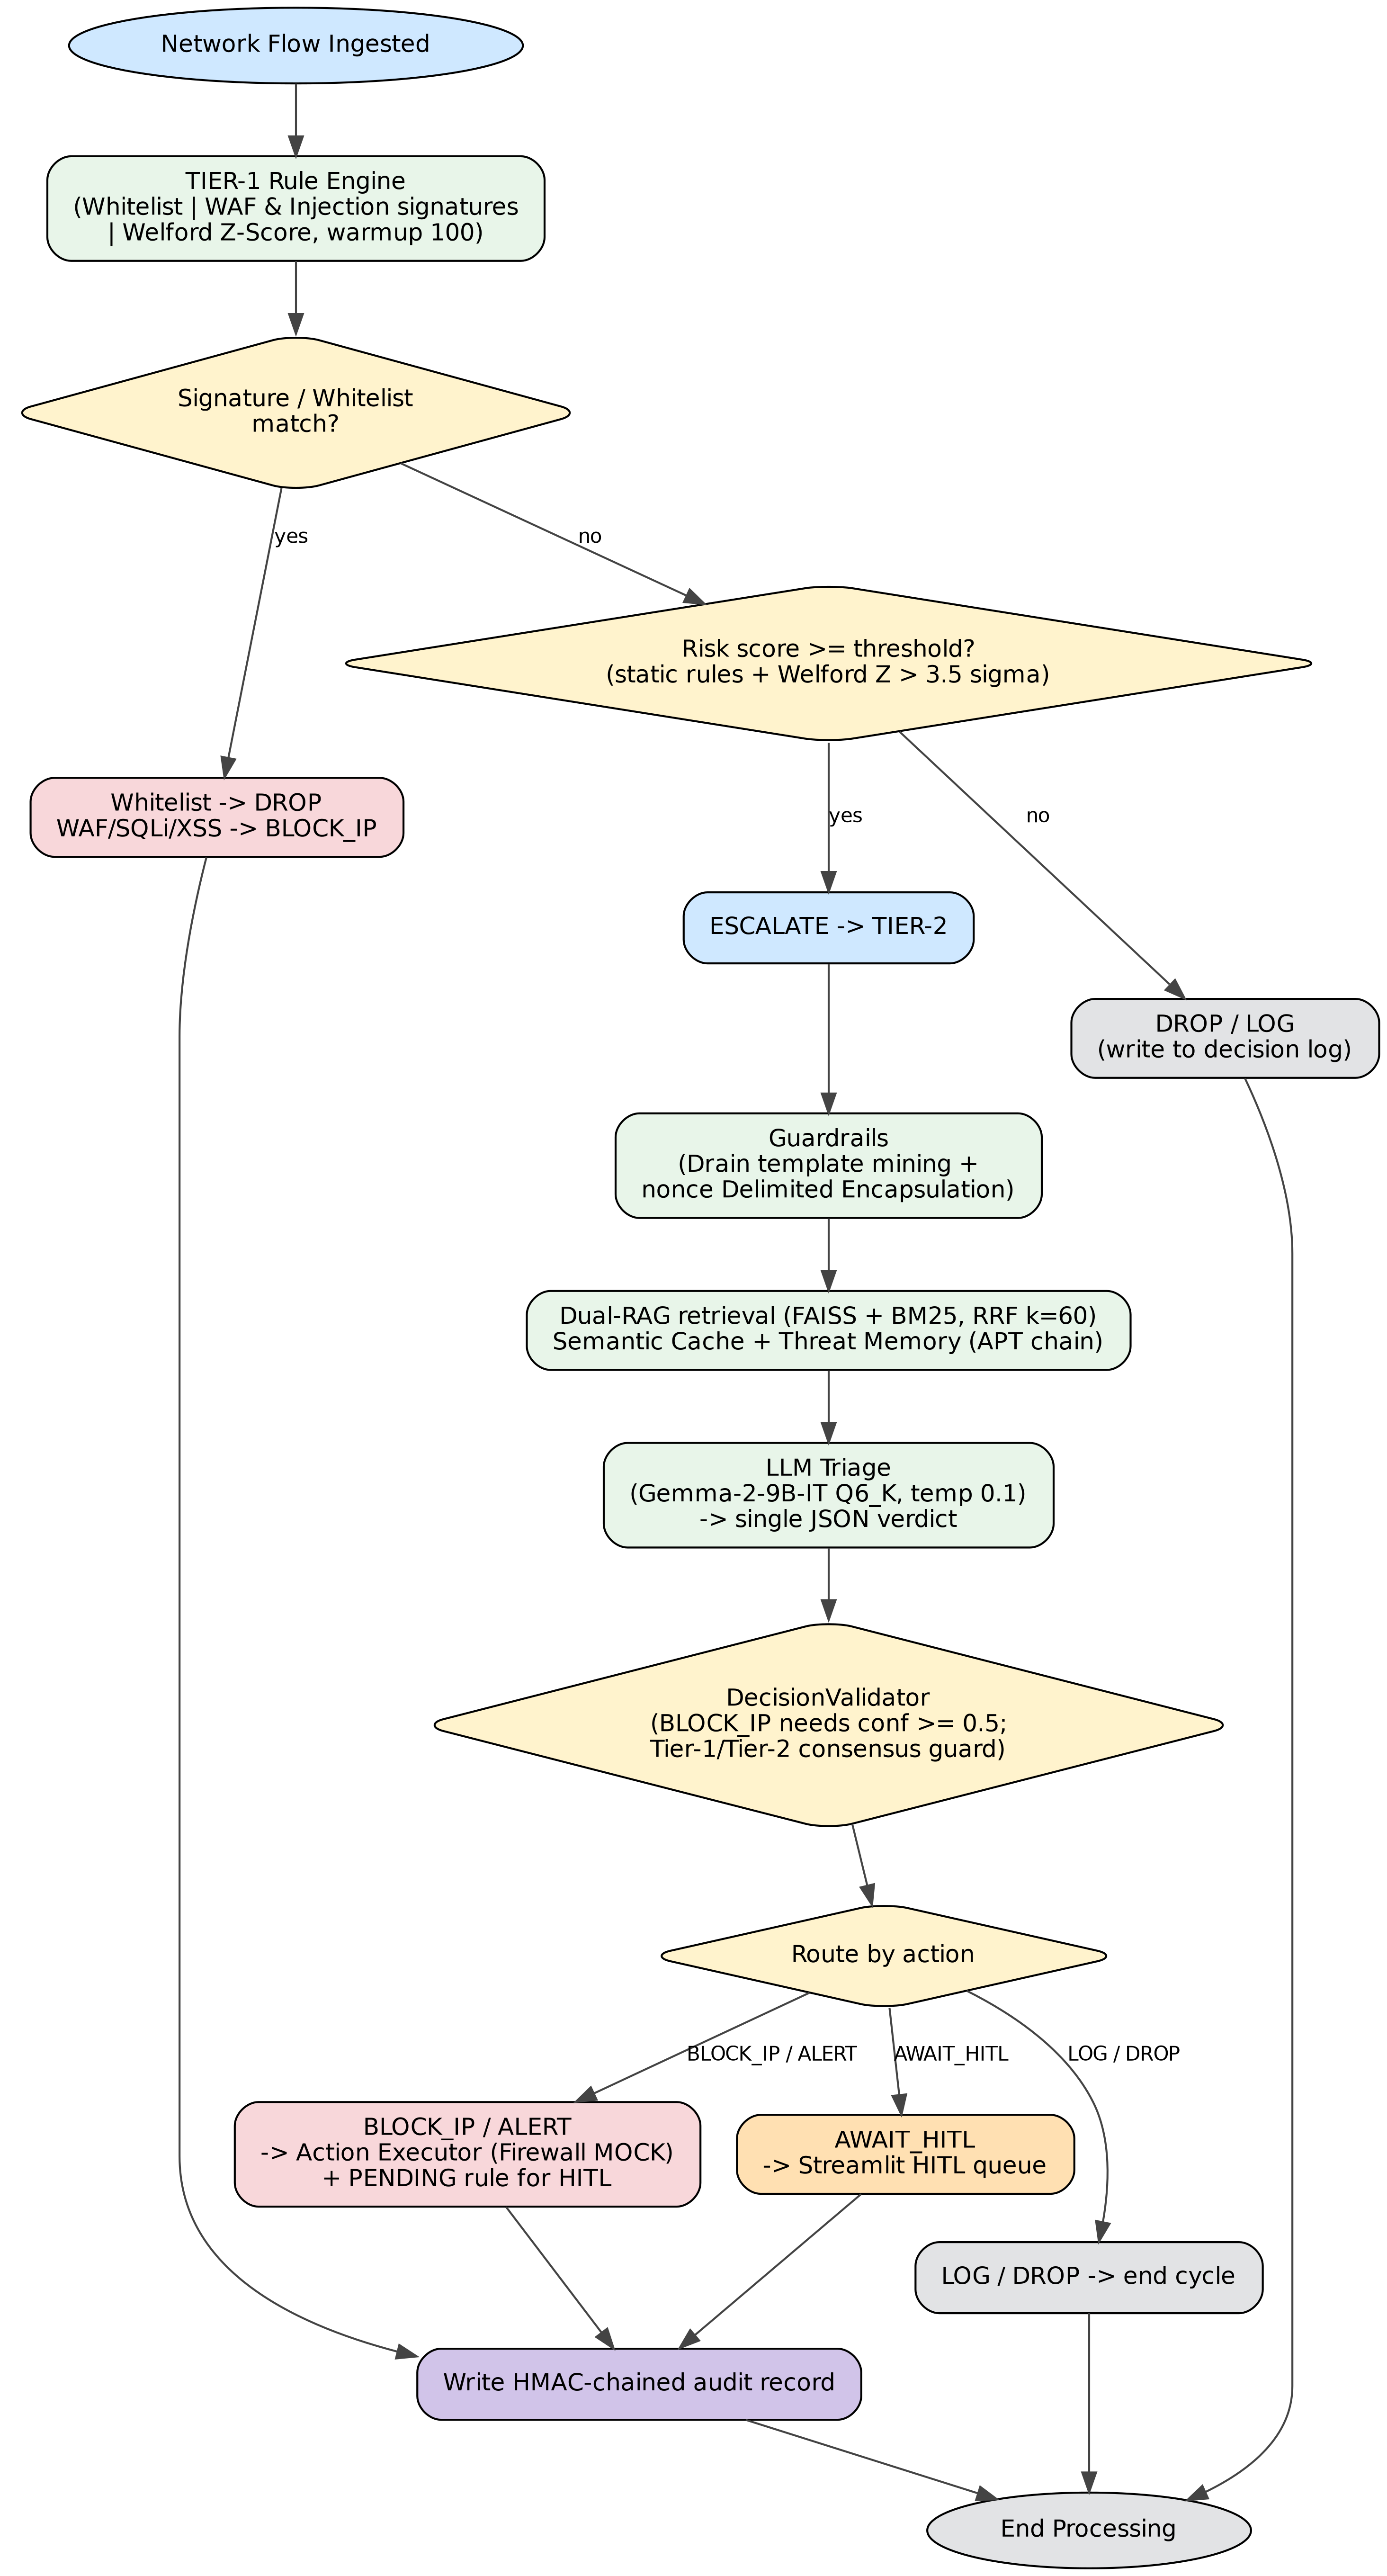
\includegraphics[width=0.95\textwidth,height=0.74\textheight,keepaspectratio]{images/sentinel_flow.png}
    \caption{Detailed operational execution flow in the SENTINEL pipeline. (Source: Author)}
    \label{fig:sentinel_flow}
\end{figure}

\section{Tier-1: Statistical Pre-filter \& ML Gateway}
Instead of forcing the LLM to process 100\% of the traffic, Tier-1 absorbs over 80\% of the volume.
\begin{itemize}
    \item \textbf{(1) Welford Algorithm:} Computes real-time Z-scores per IP to detect anomalies without retaining entire datasets in memory.
    \item \textbf{ML Gateway (LightGBM):} Assigns risk scores. Extremely high-risk cases ($>0.85$) are blocked instantly, sparing LLM resources.
    \item \textbf{Semantic Cache (Tier 1.75):} Caches LLM resolutions for malicious payloads using SHA-256 hashes. Recurring payloads (e.g., Brute-force, DDoS) are blocked within 1 millisecond without LLM invocation.
\end{itemize}

\section{Tier-2: Agentic AI and State Flow (LangGraph)}
The LLM is orchestrated via a "State Graph" (LangGraph), functioning as a finite state machine (Table~\ref{tab:agent_fsm_transitions}). This strictly limits AI hallucinations by enforcing rigid workflow milestones.

\begin{table}[!htbp]
    \centering
    \caption{State transition matrix of the Tier-2 cognitive agent. (Source: Author)}
    \label{tab:agent_fsm_transitions}
    \begin{tabular}{|>{\raggedright\arraybackslash}p{0.20\textwidth}|>{\raggedright\arraybackslash}p{0.27\textwidth}|>{\raggedright\arraybackslash}p{0.18\textwidth}|>{\raggedright\arraybackslash}p{0.16\textwidth}|}
        \hline
        \textbf{State} & \textbf{Input / Condition} & \textbf{Next} & \textbf{Action} \\
        \hline
        \texttt{GUARDRAILS} & Receive batch & \texttt{RAG\_CONTEXT} & Compress \& wrap \\ \hline
        \texttt{RAG\_CONTEXT} & Context retrieval & \texttt{LLM\_TRIAGE} & Add MITRE/NIST \\ \hline
        \texttt{LLM\_TRIAGE} & Action decision & \texttt{ATTACK\_MAPPER} & MITRE mapping \\ \hline
        \texttt{ATTACK\_MAPPER} & \texttt{BLOCK}/\texttt{ALERT} & \texttt{ACTION\_EXEC} & Block/Alert \\ \hline
        \texttt{ATTACK\_MAPPER} & \texttt{AWAIT\_HITL} & \texttt{HITL} & Escalate to Analyst \\ \hline
    \end{tabular}
\end{table}

\section{Knowledge Retrieval (Dual-RAG) and Memory}
To ensure highly specialized decisions, SENTINEL utilizes a hybrid RAG mechanism, fusing Vector search (semantic) and BM25 (keyword) via Reciprocal Rank Fusion (Table~\ref{tab:search_comparison}). The knowledge source comprises MITRE ATT\&CK and NIST frameworks.

\begin{table}[!htbp]
    \centering
    \caption{Retrieval models in the hybrid search strategy (Dual-RAG). (Source: Author)}
    \label{tab:search_comparison}
    \begin{tabular}{|>{\raggedright\arraybackslash}p{0.20\textwidth}|>{\raggedright\arraybackslash}p{0.31\textwidth}|>{\raggedright\arraybackslash}p{0.31\textwidth}|}
        \hline
        \textbf{Dimension} & \textbf{Dense (FAISS / Vector)} & \textbf{Sparse (BM25 / Keyword)} \\
        \hline
        Model & all-MiniLM-L6-v2 & BM25 Weights \\ \hline
        Strengths & Understands semantics, concepts & Exact IDs (CVE, IP) \\ \hline
    \end{tabular}
\end{table}

\textbf{Threat Memory:} Used to correlate persistent attacks (APT) across time. IP reputation degrades over multiple days. If the score hits a critical threshold (100), the IP is automatically blocked at the network edge (Tier-1).

\begin{table}[!htbp]
    \centering
    \caption{Threat Memory Database Schema. (Source: Author)}
    \label{tab:threat_memory_schema}
    \begin{tabular}{|>{\raggedright\arraybackslash}p{0.24\textwidth}|>{\raggedright\arraybackslash}p{0.34\textwidth}|>{\raggedright\arraybackslash}p{0.28\textwidth}|}
        \hline
        \textbf{Table} & \textbf{Primary Key} & \textbf{Purpose} \\
        \hline
        \texttt{ip\_reputation} & \texttt{ip} (PK), \texttt{reputation\_score} & Long-term IP reputation. \\ \hline
        \texttt{threat\_events} & \texttt{id}, \texttt{src\_ip}, \texttt{label} & Multi-day APT correlation. \\ \hline
    \end{tabular}
\end{table}

\section{Prompt Injection Defense and Transparency}
Every payload ingested by the LLM is wrapped in random cryptographic nonces (e.g., \texttt{<<<DATA\_8F3E...>>>}). This signals the LLM that the enclosed content is purely passive data, forbidding the execution of any hidden instructions. Finally, every verdict is hashed (HMAC-SHA256) into an audit chain; any retrospective tampering breaks the chain, triggering immediate Dashboard alerts.
